\documentclass{homework}


\usepackage{rail} % Draw syntax, cfg diagram
\railalias{curlL}{\{}
\railalias{curlR}{\}}
\railalias{arrow}{->}

\definecolor{bg}{rgb}{0.95,0.95,0.95}

\begin{document}
\frontpage{Þýðendur}{Parser-NanoMorpho}{Guðmundur Óli Norland}{Egill Ragnarsson}{Snorri Agnarsson}

\begin{question}{Github}
  \href{https://github.com/slowpokesheep/thydendur/blob/master/nanomorpho/Parser.java}{Parser}\\
\end{question}

\begin{question}{Parser.java}
\end{question}
\begin{answer}
\begin{minted}[autogobble,tabsize=2, bgcolor=bg,breaklines,breakanywhere]{java}
import java.io.FileReader;
import java.io.IOException;

public class Parser {
  private static NanoMorpho lexer;
  private static int token;

  private static boolean should_advance = true;

  public static void main(String[] args) throws Exception {
    lexer = new NanoMorpho(new FileReader(args[0]));
    token = advance();

    while (token != 0) {
      func();
      token = lexer.yylex();
    }
    System.out.println("Accepted!");
  }

  private static void debug(int line) {
    System.out.println("DEBUG: line-" + line + ", token-" + token + ", lexeme-" + lexer.getLexeme());
  }

  // Print error message
  private static void error(String s) {
    throw new Error(
        "Line " + lexer.getLineNumber() +
        ": Expected " + s + " but found " + lexer.getLexeme()
    );
  }

  private static String errorMsg(int expected) {
    switch (expected) {
      case NanoMorpho.NAME: return "name";
      default: return "unknown";
    }
  }

  private static int asciiValue(char c) {
    return (int) c;
  }

  // Check if token is valid
  private static void check(int expected) {
    if (token != expected) error(errorMsg(expected));
  }

  // Check if token is valid
  private static void check(char expected) {
    if (token != (asciiValue(expected))) error(""+expected);
  }

  // Optional check for token
  private static boolean optionalCheck(int opt) {
    if (token != opt) return false;
    return true;
  }

  // Optional check for token
  private static boolean optionalCheck(char opt) {
    if (token != asciiValue(opt)) return false;
    return true;
  }

  private static int advance() throws Exception {
    if (should_advance) {
      token = lexer.yylex();
      if (token == 0) {
        throw new Error("Ending is invalid");
      }
    }
    should_advance = true;
    return token;
  }

  /* 
    we look at the next token without "using" it,
    meaning that the next time advance is called,
    the same token is used
  */
  private static int lookahead() throws Exception {
    advance();
    should_advance = false;
    return token;
  }

  public static void func() throws Exception {
    // *** NAME(... , ...) *** //
    check(NanoMorpho.NAME);
    
    // Read next token
    advance();
    check('(');
    
    // Read next token
    advance();
    

    if (! optionalCheck(')')) {
      
      check(NanoMorpho.NAME);

      // Read next token
      advance();

      // Reading function parameters
      while (optionalCheck(',')) {

        // Read next token
        advance();
        check(NanoMorpho.NAME);

        // Read next token
        advance();
      }
      
    }

    // Closing function paranthesis
    check(')');
    
    // Read next token
    advance();
    check('{');

    // *** { decl;* expr;*} *** //
    decl();
    
    /* 
      we check for expressions until we reach },
      or we reach an invalid ending.
      We also want to make sure the function contains
      at least one expression.
    */    
    boolean contains_expr = false;

    while (! optionalCheck('}')) {
      expr();

      // Read next token
      advance();
      check(';');

      // Read next token
      advance();
      contains_expr = true;
    }
    if (!contains_expr) error("expression");
  }

  // *** var NAME,NAME..... *** //
  public static void decl() throws Exception {

    // just in case it's set to false before the call
    should_advance = true;

    // Lookahead next token
    lookahead();
    
    while (optionalCheck(NanoMorpho.VAR)) {

      // Use token
      advance();

      // Read next token
      advance();
      check(NanoMorpho.NAME);

      // Additional variables, seperate by commas
      advance();
      while (optionalCheck(',')) {

        // Read next token
        advance();
        check(NanoMorpho.NAME);

        advance();
      }
      check(';');

      // Lookahead next token
      lookahead();
    }
  }

  public static void expr() throws Exception {

    // just in case it's set to false before the call
    should_advance = true;

    boolean is_empty = true;
    
    // *** NAME | NAME = expr | NAME = (expr,....) *** //
    if (optionalCheck(NanoMorpho.NAME)) {
      
      // assigning to a variable => NAME = expr
      
      // Lookahead next token
      lookahead();

      if (optionalCheck('=')) {

        // Read next token
        advance();
        advance();

        expr();
      }
      
      // Lookahead next token
      lookahead();

      if (optionalCheck('(')) {

        // Read next token
        advance();
        // Lookahead next token
        lookahead();

        if (! optionalCheck(')')) {

          // First parameter
          advance();
          expr();

          // Additional parameters
          advance();
          while (optionalCheck(',')) {
            // n parameter
            advance();
            expr();
          }

          // Read next token
          advance();
          check(')');

        }
        else advance();

      }
      is_empty = false;
    }

    // *** return expr | OPNAME expr *** //
    else if (optionalCheck(NanoMorpho.RETURN) || optionalCheck(NanoMorpho.OPNAME)) {
      
      // Read next token
      advance();
      expr();
      is_empty = false;
    }

    // *** LITERAL *** //
    else if (optionalCheck(NanoMorpho.LITERAL)) is_empty = false;


    else if (optionalCheck('(')) {
      
      // Read next token
      advance();
      expr();

      // Read next token
      advance();
      check(')');

      is_empty = false;
    }

    else if (optionalCheck(NanoMorpho.WHILE)) {

      // Read next token
      advance();
      check('(');
      
      // Read next token
      advance();
      expr();

      // Read next token
      advance();
      check(')');

      body();
      is_empty = false;
    }
    else is_empty = ifexpr();

    // Empty expressions result in an error
    if (is_empty) error("expression");

    // Lookahead and check if next token is an operator, if so
    // we need to follow up with an expression
    lookahead();
    
    if (optionalCheck(NanoMorpho.OPNAME)) {

      advance();

      // Read next token
      advance();
      expr();
    }
  }

  // Returns true if the ifexpr is empty
  public static boolean ifexpr() throws Exception {
    
    // just in case it's set to false before the call
    should_advance = true;
    
    if (optionalCheck(NanoMorpho.IF)) {

      // Read next token
      advance();
      check('(');
      
      // Read next token
      advance();
      expr();

      // Read next token
      advance();
      check(')');

      body();

      // Lookahead next token
      lookahead();
      if (optionalCheck(NanoMorpho.ELSIF)) {

        // Use token
        advance();

        // Read next token
        advance();
        check('(');

        // Read next token
        advance();
        expr();

        // Read next token
        advance();
        check(')');

        body();
      }
      
      // Lookahead next token
      lookahead();
      if (optionalCheck(NanoMorpho.ELSE)) {

        // Use token
        advance();
        body();
      }
      return false;
    }
    return true;
  }

  public static void body() throws Exception {    
    
    // just in case it's set to false before the call
    should_advance = true;

    // Read next token
    advance();
    check('{');

    while (! optionalCheck(';')) {

      advance();
      expr();
      advance();
    }

    // Read next token
    advance();
    check('}');
  }

}
\end{minted}
\end{answer}

\newpage

\begin{question}{NanoMorpho-Málrit}
\end{question}
\begin{answer}
  \begin{rail}
    program : ( function + )
  \end{rail}
  \begin{rail}
    function  : NAME '('  ( NAME + ',' ) ? ')' ;
    arrow     : curlL ( decl ';' + ) ? ( expr ';' + ) curlR ;
  \end{rail}
  \begin{rail}
    decl : 'var' ( NAME + ',' )
  \end{rail}
  \begin{rail}
    expr  : NAME
          | NAME '=' expr
          | NAME '('  ( expr + ',' ) ?   ')'
          | 'return' expr
          | OPNAME expr
          | expr OPNAME expr
          | LITERAL
          | '('  expr  ')'
          | ifexpr
          | 'while' '('  expr  ')' body
  \end{rail}
  \begin{rail}
    ifexpr  : 'if' '('  expr  ')' body ;
    arrow   : (  ( 'elsif' '('  expr  ')'  body  + )  ) ? ;
    arrow   : ( 'else' body ) ? ;
  \end{rail}
  \begin{rail}
    body : curlL ( expr ';' + ) curlR
  \end{rail}
\end{answer}

\begin{question}{Test output}
  \textbf{\underline{Test Invalid 1}}
  \begin{verbatim}
    main(asd {

    error -> paranthesis left open
  \end{verbatim}
  \textbf{\underline{Test Invalid 2}}
  \begin{verbatim}
    main() {
      var z;
    }

    error -> no expression in function
  \end{verbatim}
  \textbf{\underline{Test Invalid 3}}
  \begin{verbatim}
    main() {
      var x, y, z, asd, qwe;
      x = y = z = 123;
      asd =;
      error -> no variable assignment
    }
  \end{verbatim}
  \textbf{\underline{Test Invalid 4}}
  \begin{verbatim}
    main() {
      var x;
      x = x + x + x +;
      error -> end of line operator
    }
  \end{verbatim}
  \textbf{\underline{Test Invalid 5}}
  \begin{verbatim}
    main(asd, qwe, sdf) {
      if () {
        error -> not if statement expression
      };
    }
  \end{verbatim}
  \textbf{\underline{Test Invalid 6}}
  \begin{verbatim}
    (asd) {
      var hallo = 1;
    }
    error -> No function name
  \end{verbatim}
  \textbf{\underline{Test Valid}}
  \begin{verbatim}
    main(asd, sdf) {
      var krabbi;
      var bubbi;
      bubbi();
      while(x == 5) {
        bubbi();
      };
      if (krabbi != 123 != asd < bvc) {
        if (x) {
          while (z > asdfghjkl) {
            return 5;
          };
        };
      };
      return 0;
    }
    
    epli(lol) {
      var epli;
      epli = (567 - 123) + (999 && 345);
      mango;
      if (5 > 6) {
        1 + 2;
      } elsif (6 > 7) {
        2 + 3;
      } else {
        1 + 2 * 3;
      };
    }    
  \end{verbatim}
\end{question}
\begin{answer}
  \begin{figure}[h]
    \centering
    \caption*{Test}
    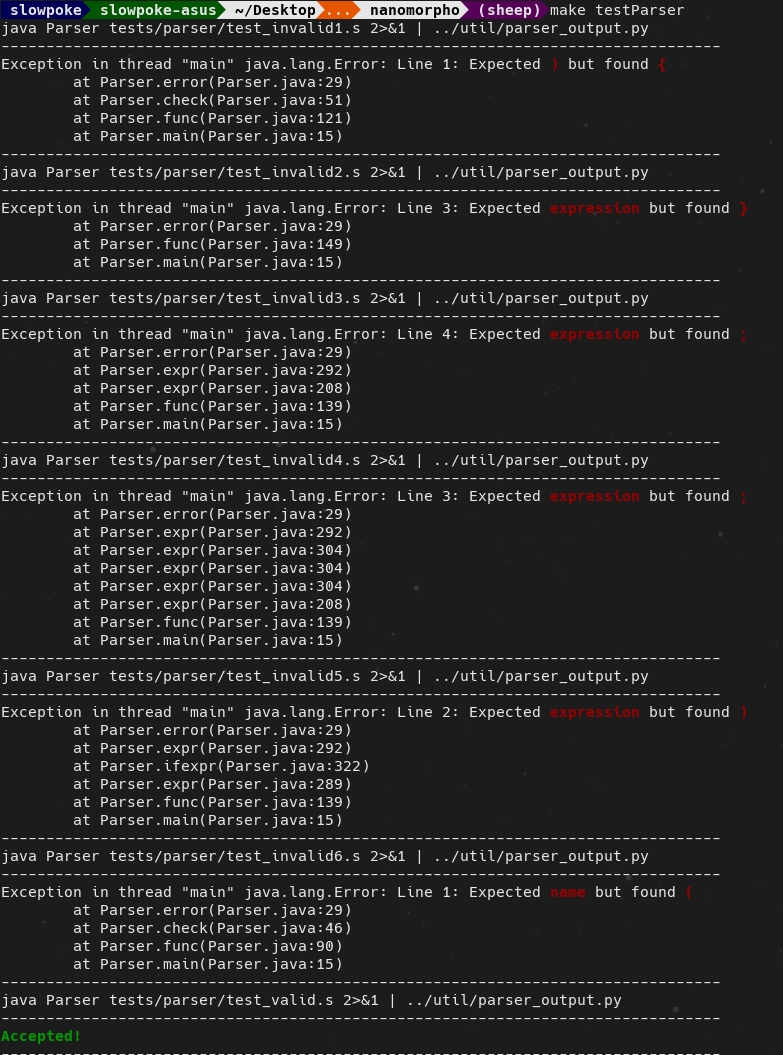
\includegraphics[width=0.8\textwidth]{testParser.png}
  \end{figure}
\end{answer}

\end{document}
